\documentclass[a4paper]{article}

\usepackage[table]{xcolor}%this has to be the first!!!!!!
\usepackage{fullpage} % Package to use full page
%\usepackage{parskip} % Package to tweak paragraph skipping
\usepackage{tikz} % Package for drawing
\usepackage{tikz-3dplot} % Package for drawing
\usetikzlibrary{shapes,arrows,matrix,positioning}
\usepackage{amsmath}
\usepackage{indentfirst}
\usepackage{hyperref}
\usepackage{subcaption}
\usepackage{graphics}
\usepackage{graphicx}
\usepackage{minted}
\usepackage{romannum}
\AtBeginDocument{\pagenumbering{arabic}}% To keep page number arabic
\usepackage{multicol}
\usepackage{mathrsfs}
%color define
\definecolor{codebg}{RGB}{230,255,253}
\definecolor{function}{RGB}{210,0,26}
\definecolor{para}{RGB}{255,137,137}
\definecolor{output}{RGB}{238,224,201}
\setminted[cpp]{mathescape=true,breaklines,bgcolor=codebg,linenos}

\tikzset{
  block/.style = {rectangle, draw, fill=output, text width=6cm, text centered, rounded corners, minimum height=4em},
  line/.style = {draw, -latex'},
}

%function newcommand
\newcommand{\func}[1]{\textbf{\textcolor{function}{#1}}}
\newcommand{\para}[1]{\textbf{\emph{\textcolor{para}{#1}}}}
\newcommand{\activetest}{\tikz \fill[black] (3pt,3pt) circle (3pt);}
\newcommand{\prolong}{\tikz \fill[blue] (3pt,3pt) circle (3pt);}
\newcommand{\rest}{\tikz \fill[red] (3pt,3pt) circle (3pt);}

\usepackage{biblatex}
\addbibresource{bibliography.bib}
\title{poisson.h Documentation}
\author{Haochen(Langford) Huang}
\date{\today}

\makeatletter%title setting
\def\@maketitle{%
  \newpage
  \null
  \vskip 2em%
  \begin{center}%
  \let \footnote \thanks
    {\LARGE \@title \par}%
    \vskip 1.5em%
    {\Large
      \lineskip .5em%
      \begin{tabular}[t]{c}%
        \@author
      \end{tabular}\par}%
    \vskip 1em%
    {\large \@date\par}%
    \vskip 1em%
    {\large version:1.0}%
  \end{center}%
  \par
  \vskip 1.5em}
\makeatother

\begin{document}

\maketitle

\section{Introduction and Background}\label{sec:intro}
\textbf{poisson.h} serves as toolbox which provides functions to construct V-cycle iteration solver for implicit equations. A specific one for solving poisson equation is constructed within the headfile as an example. We shall first introduce the constructing toolbox.\par
Assuming the governing equation can be written as
\begin{equation}
  f( x) = y
\end{equation}
where $y$ is the known variable, $ x$ is the desired variable and $f$ represents linear operator that satisfies
\begin{equation}\label{equ:cons}
  f( x_a+ x_b) = f( x_a) + f( x_b)
\end{equation}
Now consider the discrete form of operator $\hat{f}$ which takes all desired variable from every cell (suppose the total number of cell is $n$) to express the local known variable $y_i$ then yields the implicit equation group
\begin{equation}\label{equ:aim}
  \hat{f}(x_1,x_2,x_3,\cdots,x_n) = y_i \quad i = 1,2,\cdot,n
\end{equation}
which can be solved by indirective iterative method such as Jacobi method, G-S method\cite{moin2010fundamentals} \emph{etc.} Moreover, constraints \ref{equ:cons} provide another perspective to construct equation group. Use $x_1^e,x_2^e,\cdots,x_n^e$ to denote exact solution of equation \ref{equ:aim} and $x_1^k,x_2^k,\cdots,x_n^k$ to represent result of $k$th iteration. Following equation \ref{equ:cons} we have
\begin{equation}\label{equ:iter}
  \hat{f}(\delta x_1^k,\delta x_2^k,\cdots, \delta x_n^k) = RES^k
\end{equation}
where $\delta x_i^k = x_i^e - x_i^k$, $RES^k = \hat{f}(x_1^e,x_2^e,\cdots,x_n^e) - \hat{f}(x_1^k,x_2^k,\cdots,x_n^k)$. The criterion of solution then becomes $|RES^k|_{\infty}<\epsilon$ where $\epsilon$ is a setting tolerance.\par
There are many techniques to accelerate the convergence of iteration, and multigrid method\cite{wesseling1995introduction} may be one of the most famous which employs iterations on every layer of the mesh to reduce the residual of corresponding wavenumber. A similar methodology is applied by quadtree/octree in Basilisk. Take quadtree as an exapmle. Consider tree architecture in Fig.\ref{fig:2dquad}, the actual calculating rules for this problem is shown in \ref{fig:caculation} where $\activetest$ represents leaf cells (the finest cell at this area and is not divided by higher level) and the value it carrying is the the final value shown in the result called active value.
$\prolong$ represents ghost cell served as boundary condition whose value is computed by bilinear interpolation. Finally $\rest$ represents value carried by parent cell. The parent cell, indicated by its name, will be divided into 4(8) children cells in finer layer (level in Basilisk).\cite{van2018towards}\par
A single round of iteration is accomplished by two procedures. First, from highest level to lowest one, assign residual to each cell of current level which form the \emph{R.H.S.} of equation \ref{equ:iter}. Second, starting from lowest level to the highest, obtain the result after few iterating (by Jacobi method or GS method) on current level and use it to compute initial value on next level. We shall first dive into second procedure which is more sophisticated.\par
Calculations happens at every level shown in Fig.\ref{fig:caculation}, when it comes to higher level the boundary condition is first set and then undergoes the iteration on cells at same level instead of whole domain. Moreover, the initial value on each level is obtained by prolongation (bilinear mostly) from previous mesh level.\par
In order to facilitate equation \ref{equ:iter} we also need residual, which only exists at leaf cell, of every cell at each level. This procedure is achieve by restricting\cite{popinet2015quadtree} (averaging mostly) value on 4(8) children cells, which is much simpler compared to bilinear that use in previous description.\par 
\begin{figure}[h]
  \begin{subfigure}[b]{0.5\textwidth}
    \centering 
    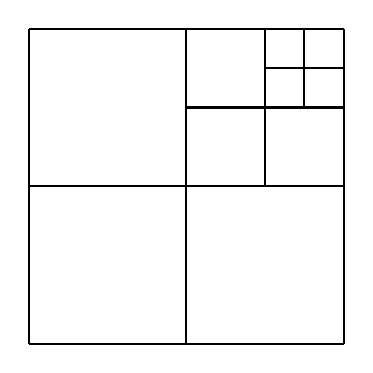
\begin{tikzpicture}
      \draw[thick,step=2cm] (0,0) grid (4,4);
      \draw[thick,step=1cm] (2,2) grid (4,4);
      \draw[thick,step=0.5cm] (3,3) grid (4,4);
    \end{tikzpicture}
    \caption{2D quadtree example.}
    \label{fig:2dquad}
  \end{subfigure}
  \begin{subfigure}[b]{0.5\textwidth}
    \centering 
    \tdplotsetmaincoords{70}{110}
    \begin{tikzpicture}[tdplot_main_coords]
      \foreach \i in {0,2,4}
      {
        \draw[thick] (\i,0,4.5) -- (\i,4,4.5);
        \draw[thick] (0,\i,4.5) -- (4,\i,4.5);
      }
      
      \foreach \i in {1,3}
      {
        \filldraw[black] (1,\i,4.5) circle (2.5pt);
        \filldraw[black] (3,\i,4.5) circle (2.5pt);
      }
      \filldraw[red] (3,3,4.5) circle (2.5pt);

      \foreach \i in {2.5,3.5}
      {
        \draw[gray,dashed] (3,3,4.5)--(\i,2.5,3);
        \draw[gray,dashed] (3,3,4.5)--(\i,3.5,3);

        \filldraw[black] (\i,2.5,3) circle (2pt);
        \filldraw[black] (\i,3.5,3) circle (2pt);

        \filldraw[blue] (\i,1.5,3) circle (2pt);
        \filldraw[blue] (\i,4.5,3) circle (2pt);
        \filldraw[blue] (1.5,\i,3) circle (2pt);
        \filldraw[blue] (4.5,\i,3) circle (2pt);
      }

      \filldraw[red] (3.5,3.5,3) circle (2pt);

      \foreach \i in {2,3,4}
      {
        \draw[thick] (\i,2,3) -- (\i,4,3);
        \draw[thick] (2,\i,3) -- (4,\i,3);
      }

      \foreach \i in {3.25,3.75}
      {
        \draw[gray,dashed] (3.5,3.5,3)--(\i,3.25,1.75);
        \draw[gray,dashed] (3.5,3.5,3)--(\i,3.75,1.75);
        \filldraw[black] (\i,3.25,1.75) circle (1pt);
        \filldraw[black] (\i,3.75,1.75) circle (1pt);

        \filldraw[blue] (\i,2.75,1.75) circle (1pt);
        \filldraw[blue] (\i,4.25,1.75) circle (1pt);
        \filldraw[blue] (2.75,\i,1.75) circle (1pt);
        \filldraw[blue] (4.25,\i,1.75) circle (1pt);
      }

      \foreach \i in {3,3.5,4}
      {
        \draw[thick] (\i,3,1.75) -- (\i,4,1.75);
        \draw[thick] (3,\i,1.75) -- (4,\i,1.75);
      }

      \draw[very thick,-latex] (3,1,3.5)--(3,1,1.0);
    \end{tikzpicture}
    \caption{Calculation for each level. }
    \label{fig:caculation}
  \end{subfigure}
    \caption{Quadtree example. Arrow in (b) indicates calculating sequence.}
    \label{fig:2dexample}
\end{figure}
After introducing the mesh architecture, we shall now step a little further to see the solver structure provided by 'poisson.h' and to perceive the overall workflow. FIG.\ref{fig:workflow} displays whole system as well as its workflow. As can be seen from the sketch, the whole solver consists of four functions, \func{mg\_solve}, \func{mg\_cycle}, \func{relax} and \func{residual}. Their nesting relating is shown by corresponding position, \emph{e.g.} \func{relax} is inside \func{mg\_cycle} while \func{residual} and \func{mg\_cycle} locate inside \func{mg\_solve} indicates that \func{relax} is called by \func{mg\_cycle} and \func{mg\_cycle} along with \func{residual} are directly called by \func{mg\_solve}. Detailed workflow is also presented, after inputting $ \mathbf{x}^0, \mathbf{y}$ before the residual actually meet the tolerance $\epsilon$, \func{mg\_solve} plays as a manager to make rest functions coordinate, $ \mathbf{x}^k$ is conveyed between \func{mg\_cycle} and \func{residual} to renew. Number behind each step represents the order within the loop. $ \mathbf{x}^k, \mathbf{y}$ is first sent to residual to compute residual $RES^k$ which served as parameter in \func{mg\_cycle}. $ \mathbf{x}^k$ and $n$ are also taken into \func{mg\_cycle} where $n$ controls iteration number on each mesh level. $ \mathbf{x}^{k+1}$ is obtained by first solving equation \ref{equ:iter} for $\delta \mathbf{x}^k$ then execute update
\begin{equation}
  \mathbf{x}^{k+1} = \mathbf{x}^k + \delta \mathbf{x}^{k+1}
\end{equation}
Loop will break out either residual satisfies tolerance constraint or number of round exceed setting threshold. Readers may notice there is no parameters conveyed within \func{mg\_cycle}, this is because relationship between \func{relax} and \func{mg\_cycle} cannot be simply abstracted as 'linear' as depicted in this figure. Structure inside \func{mg\_cycle} is demonstrate in Fig.\ref{fig:mgcycle} as described before residual is assigned to each level then relax is called at each level multiple times updating $\delta \mathbf{x}^k$ in the form (condition varies according to iteration method)
\begin{equation}\label{equ:indirect}
  \delta x^{k+1}_i = F(\delta x^k_1,\delta x^k_2,\cdots,\delta x^k_{i-1},\delta x^k_{i+1},\cdots,\delta x_n^k, RES^k)
\end{equation}
Back to \func{mg\_solve}, readers may notice from Fig.\ref{fig:workflow} that all the function within, including \func{mg\_solve} itself, are divided into three layer by dashed line and each layer is named by Roman number from top to bottom. Higher the layer, more irreplaceable the function is. Therefore, functions at \Romannum{3} can be changed or altered based on one's purpose. In another word, users can choose their own \func{relax} and \func{residual} based on equation they cope with. The governing equation for \textbf{poisson.h} is
\begin{equation}\label{equ:poisson}
  L(a)=\nabla\cdot(\alpha\nabla a) + \lambda a =b
\end{equation}
where $L$ is a linear operator. Based on above discussion such equation can be solved by multigrid solver only if one constructs appropriate \func{relax} and \func{residual} function. Another example is referred to headfile \textbf{viscosity.h} where same solver construction is used for totally different linear equation. 

\begin{figure}[H]
    \centering
    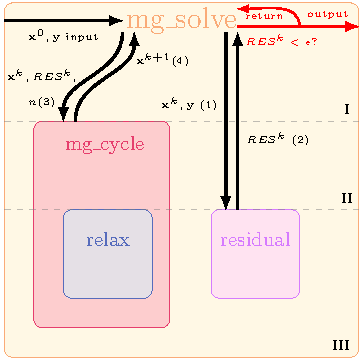
\includegraphics[width=\textwidth]{image/mgsolver.pdf}
    \caption{Architecture of the solver. Nested relationship of functions is indicated by box containing relationship \emph{e.g.} \func{mg\_cycle} contains \func{relax} but not \func{residual} indicates that \func{relax} is called in \func{mg\_cycle} while \func{residual} is called in \func{mg\_solve}.}
    \label{fig:workflow}
\end{figure}

\begin{figure}[H]
    \centering
    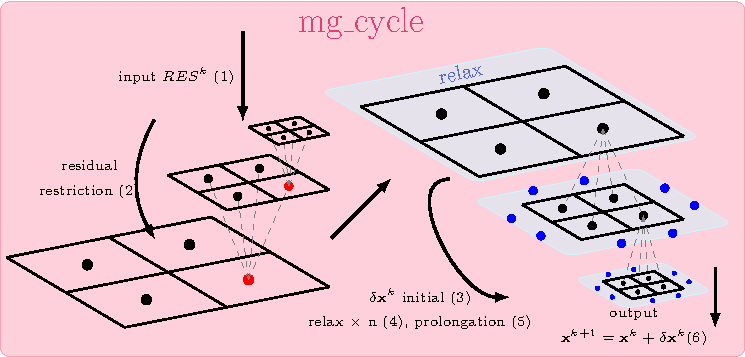
\includegraphics[width=\textwidth]{image/mgcycle.pdf}
    \caption{Combination between \func{mg\_cycle} and \func{relax}. The 'round' of iteration described before is also demonstrated in a detailed way. \func{relax} herein is embed into every level of the mesh and is executed several times (depends on parameter $n$) on each level to accelerate convergence.}
    \label{fig:mgcycle}
\end{figure}

\section{Multigrid Solver}\label{sec:mgsolver}
As indicated in section \ref{sec:intro}, we here first introduce general structure of multigrid solver which consists of \func{mg\_solve} and \func{mg\_cycle}.
\subsection{\func{mg\_cycle}}
\subsubsection{Parameters}
\begin{center}
  \begin{tabular}{|c|c|c|c|c|}
    \hline
    Name & Data type & Status & Option/Default & Representation (before/after)\\[0.5ex]
    \hline\hline
    \rowcolor{output}\para{a} & scalar* & update & compulsory & $ \mathbf{x}^{k}/ \mathbf{x}^{k+1}$\\
    \hline
    \para{res} & scalar* & unchanged & compulsory & $ \delta \mathbf{x}^k$\\
    \hline
    \para{da} & scalar* & unchanged & compulsory & $\rho^{n+ \frac{1}{2}}$\\
    \hline
    \para{relax} & void* & unchanged & compulsory &  \func{relax}\\
    \hline
    \para{data} & void* & unchanged & compulsory &  \func{Poisson} (struct defined below)\\
    \hline
    \para{nrelax} & int & unchanged & compulsory & $n$ \\
    \hline
    \para{minlevel} & int & unchanged & compulsory & $minlevel$ \\
    \hline
    \para{maxlevel} & int & unchanged & compulsory & $maxlevel$ \\
    \hline
  \end{tabular}
\end{center}

\subsubsection{Worth Mentioning Details}
As described in Sec.\ref{sec:intro} and Fig.\ref{fig:mgcycle} function \func{mg\_cycle} serves as a subcomponent to update the result. Details of such function have been explored before and shall not be repeated here.

\subsubsection{Program Workflow}
\begin{multicols}{2}
  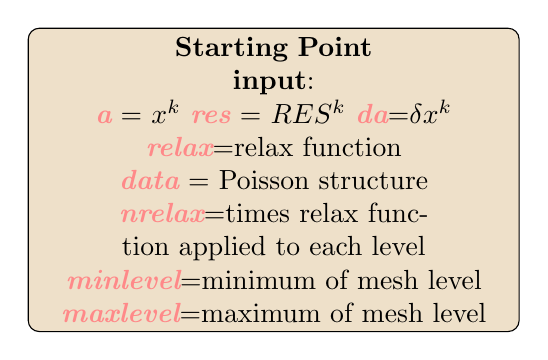
\begin{tikzpicture}
    \node [block](init){
        \textbf{Starting Point}\\
        \textbf{input}: \\
        \para{a} = $x^k$ \para{res} = $RES^k$ \para{da}=$\delta x^k$\\ \para{relax}=relax function \para{data} = Poisson structure\\
        \para{nrelax}=times relax function applied to each level\\
        \para{minlevel}=minimum of mesh level\\
        \para{maxlevel}=maximum of mesh level
      };
  \end{tikzpicture}
 \columnbreak
 \begin{minted}{cpp}
void mg_cycle (scalar * a, scalar * res, scalar * da,
	       void (* relax) (scalar * da, scalar * res, int depth, void * data),
	       void * data, int nrelax, int minlevel, int maxlevel)
{
 \end{minted}
 
\end{multicols}

\begin{center}
  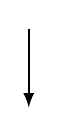
\begin{tikzpicture}
    \draw[-latex,thick](0,0) -- (0,-1); 
  \end{tikzpicture}
\end{center}

\begin{multicols}{2}
  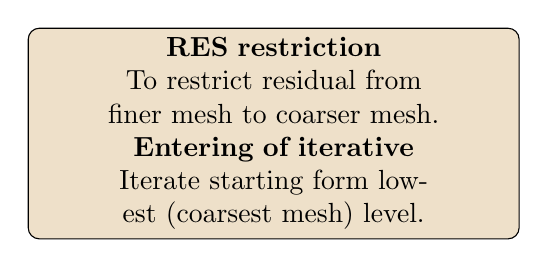
\begin{tikzpicture}
    \node [block](init){
        \textbf{RES restriction}\\
        To restrict residual from finer mesh to coarser mesh.\\
        \textbf{Entering of iterative}\\
        Iterate starting form lowest (coarsest mesh) level.
      };
  \end{tikzpicture}
  \columnbreak
  \begin{minted}{cpp}
    restriction (res);
    minlevel = min (minlevel, maxlevel);
    for (int l = minlevel; l <= maxlevel; l++) {
  \end{minted}
\end{multicols}

\begin{center}
  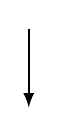
\begin{tikzpicture}
    \draw[-latex,thick](0,0) -- (0,-1); 
  \end{tikzpicture}
\end{center}

\begin{multicols}{2}
  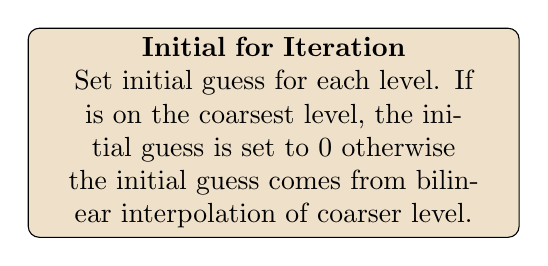
\begin{tikzpicture}
    \node [block](init){
        \textbf{Initial for Iteration}\\
        Set initial guess for each level. If is on the coarsest level, the initial guess is set to 0 otherwise the initial guess comes from bilinear interpolation of coarser level.
      };
  \end{tikzpicture}
  \columnbreak
  \begin{minted}{cpp}
    if (l == minlevel)
      foreach_level_or_leaf (l)
	for (scalar s in da)
	  foreach_blockf (s)
	    s[] = 0.;
    else
      foreach_level (l)
	for (scalar s in da)
	  foreach_blockf (s)
	    s[] = bilinear (point, s);
  \end{minted}
\end{multicols}

\begin{center}
  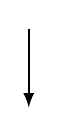
\begin{tikzpicture}
    \draw[-latex,thick](0,0) -- (0,-1); 
  \end{tikzpicture}
\end{center}

\begin{multicols}{2}
  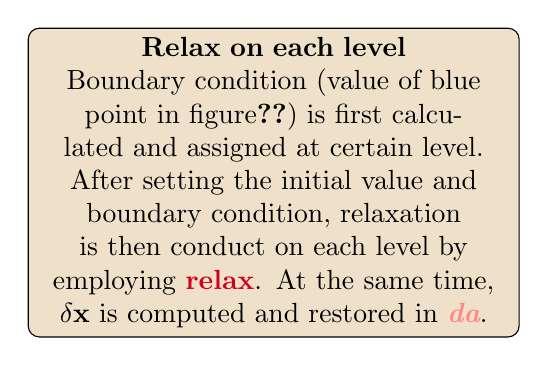
\begin{tikzpicture}
    \node [block](init){
        \textbf{Relax on each level}\\
        Boundary condition (value of blue point in figure\ref{fig:mgcycle}) is first calculated and assigned at certain level.\\
After setting the initial value and boundary condition, relaxation is then conduct on each level by employing \func{relax}. At the same time, $\delta \mathbf{x}$ is computed and restored in \para{da}. 
      };
  \end{tikzpicture}
  \columnbreak
  \begin{minted}{cpp}
    boundary_level (da, l);
    for (int i = 0; i < nrelax; i++) {
      relax (da, res, l, data);
      boundary_level (da, l);
    }
  }
  \end{minted}
\end{multicols}

\begin{center}
  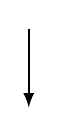
\begin{tikzpicture}
    \draw[-latex,thick](0,0) -- (0,-1); 
  \end{tikzpicture}
\end{center}

\begin{multicols}{2}
  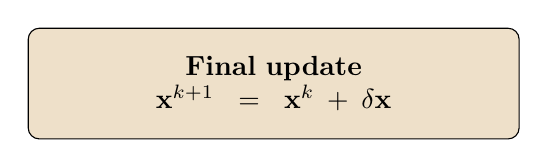
\begin{tikzpicture}
    \node [block](init){
        \textbf{Final update}\\
$\mathbf{x}^{k+1}=\mathbf{x}^k+\delta \mathbf{x}$
      };
  \end{tikzpicture}
  \columnbreak
  \begin{minted}{cpp}
  foreach() {
    scalar s, ds;
    for (s, ds in a, da)
      foreach_blockf (s)
	s[] += ds[];
  }
}
  \end{minted}
\end{multicols}

\subsection{\func{mg\_solve}}
\subsubsection{Parameters}
\begin{center}
  \begin{tabular}{|c|c|c|c|c|}
    \hline
    Name & Data type & Status & Option/Default & Representation (before/after)\\[0.5ex]
    \hline\hline
    \rowcolor{output}\para{a} & scalar* & update & compulsory & $ \mathbf{x}^{0}/ \mathbf{x}^{final}$\\
    \hline
    \para{b} & scalar* & unchanged & compulsory & $ \mathbf{y} $\\
    \hline
    \para{residual} & scalar* & unchanged & compulsory & \func{residual}\\
    \hline
    \para{relax} & void* & unchanged & compulsory &  \func{relax}\\
    \hline
    \para{data} & void* & unchanged & compulsory &  \func{Poisson} (struct defined below)\\
    \hline
    \para{nrelax} & int & unchanged & optional/4 & $n$ \\
    \hline
    \para{res} & scalar* & unchanged & compulsory & $RES$ \\
    \hline
    \para{minlevel} & int & unchanged & optional/0 & $minlevel$ \\
    \hline
    \para{tolerance} & double & unchanged & optional/$10^{-3}$ & $\epsilon$ \\
    \hline
  \end{tabular}
\end{center}
\subsubsection{Worth Mentioning Details}
Two optional components \func{residual} and \func{relax} are input as void pointer in this function. The return of this function is of self-defined data structure 'mgstats' which indeed contains information of the whole multigrid circle. The information includes \para{i}: the total number \func{mg\_cycle} is employed inside \func{mg\_solve}, \para{resb} and \para{resa}: maximum residual before/after the cycle.

\subsubsection{Program Workflow}
\begin{multicols}{2}
  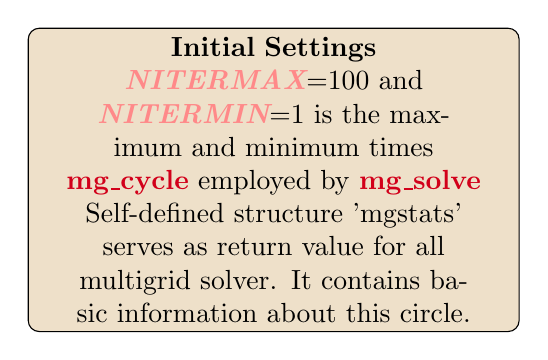
\begin{tikzpicture}
    \node [block](init){
        \textbf{Initial Settings}\\
        \para{NITERMAX}=100 and \para{NITERMIN}=1 is the maximum and minimum times \func{mg\_cycle} employed by \func{mg\_solve}\\
        Self-defined structure 'mgstats' serves as return value for all multigrid solver. It contains basic information about this circle. 
      };
  \end{tikzpicture}
 \columnbreak
 \begin{minted}{cpp}
int NITERMAX = 100, NITERMIN = 1;
double TOLERANCE = 1e-3 [*];

typedef struct {
  int i;              // number of iterations
  double resb, resa;  // maximum residual before and after the iterations
  double sum;         // sum of r.h.s.
  int nrelax;         // number of relaxations
  int minlevel;       // minimum level of the multigrid hierarchy
} mgstats;
 \end{minted}
 
\end{multicols}

\begin{center}
  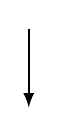
\begin{tikzpicture}
    \draw[-latex,thick](0,0) -- (0,-1); 
  \end{tikzpicture}
\end{center}

\begin{multicols}{2}
  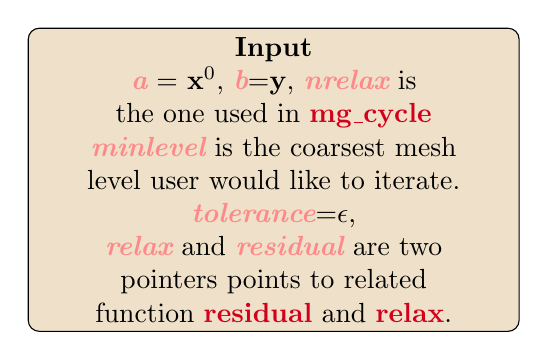
\begin{tikzpicture}
    \node [block](init){
        \textbf{Input}\\
        \para{a} = $\mathbf{x}^0$, \para{b}=$\mathbf{y}$, \para{nrelax} is the one used in \func{mg\_cycle}\\
        \para{minlevel} is the coarsest mesh level user would like to iterate.\\
        \para{tolerance}=$\epsilon$,\\
        \para{relax} and \para{residual} are two pointers points to related function \func{residual} and \func{relax}.
      };
  \end{tikzpicture}
  \columnbreak
  \begin{minted}{cpp}
mgstats mg_solve (scalar * a, scalar * b,
		  double (* residual) (scalar * a, scalar * b, scalar * res, void * data),
		  void (* relax) (scalar * da, scalar * res, int depth, void * data),
		  void * data = NULL,
		  int nrelax = 4,
		  scalar * res = NULL,
		  int minlevel = 0,
		  double tolerance = TOLERANCE)
{
   \end{minted}
\end{multicols}

\begin{center}
  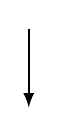
\begin{tikzpicture}
    \draw[-latex,thick](0,0) -- (0,-1); 
  \end{tikzpicture}
\end{center}

\begin{multicols}{2}
  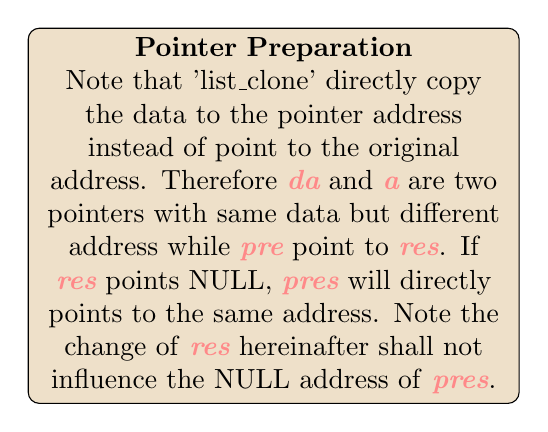
\begin{tikzpicture}
    \node [block](init){
        \textbf{Pointer Preparation}\\
        Note that 'list\_clone' directly copy the data to the pointer address instead of point to the original address. Therefore \para{da} and \para{a} are two pointers with same data but different address while \para{pre} point to \para{res}. If \para{res} points NULL, \para{pres} will directly points to the same address. Note the change of \para{res} hereinafter shall not influence the NULL address of \para{pres}. 
      };
  \end{tikzpicture}
  \columnbreak
  \begin{minted}{cpp}
  scalar * da = list_clone (a), * pres = res;
  if (!res)
    res = list_clone (b);
  \end{minted}
\end{multicols}

\begin{center}
  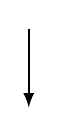
\begin{tikzpicture}
    \draw[-latex,thick](0,0) -- (0,-1); 
  \end{tikzpicture}
\end{center}

\begin{multicols}{2}
  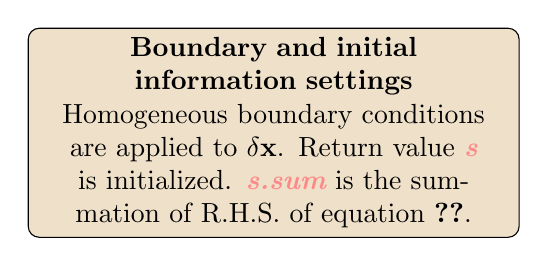
\begin{tikzpicture}
    \node [block](init){
        \textbf{Boundary and initial information settings}\\
Homogeneous boundary conditions are applied to $\delta \mathbf{x}$. Return value \para{s} is initialized. \para{s.sum} is the summation of R.H.S. of equation \ref{equ:poisson}.
      };
  \end{tikzpicture}
  \columnbreak
  \begin{minted}{cpp}
  for (int b = 0; b < nboundary; b++)
    for (scalar s in da)
      s.boundary[b] = s.boundary_homogeneous[b];

  mgstats s = {0};
  double sum = 0.;
  scalar rhs = b[0];
  foreach (reduction(+:sum))
    sum += rhs[];
  s.sum = sum;
  s.nrelax = nrelax > 0 ? nrelax : 4;
  \end{minted}
\end{multicols}

\begin{center}
  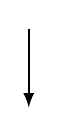
\begin{tikzpicture}
    \draw[-latex,thick](0,0) -- (0,-1); 
  \end{tikzpicture}
\end{center}

\begin{multicols}{2}
  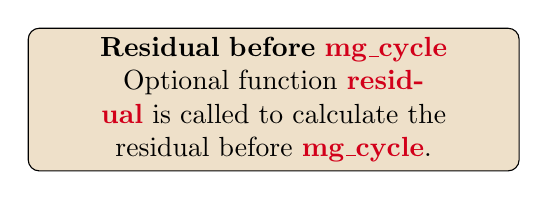
\begin{tikzpicture}
    \node [block](init){
        \textbf{Residual before \func{mg\_cycle}}\\
Optional function \func{residual} is called to calculate the residual before \func{mg\_cycle}.
      };
  \end{tikzpicture}
  \columnbreak
  \begin{minted}{cpp}
  double resb;
  resb = s.resb = s.resa = (* residual) (a, b, res, data);
  \end{minted}
\end{multicols}

\begin{center}
  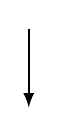
\begin{tikzpicture}
    \draw[-latex,thick](0,0) -- (0,-1); 
  \end{tikzpicture}
\end{center}

\begin{multicols}{2}
  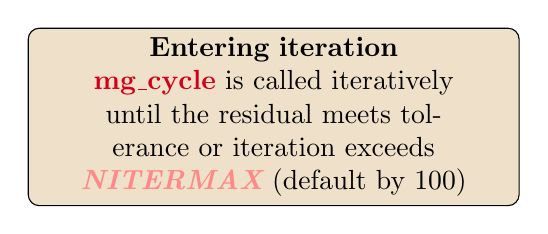
\begin{tikzpicture}
    \node [block](init){
        \textbf{Entering iteration}\\
\func{mg\_cycle} is called iteratively until the residual meets tolerance or iteration exceeds \para{NITERMAX} (default by 100)
      };
  \end{tikzpicture}
  \columnbreak
  \begin{minted}{cpp}
  for (s.i = 0;
       s.i < NITERMAX && (s.i < NITERMIN || s.resa > tolerance);
       s.i++) {
    mg_cycle (a, res, da, relax, data,
	      s.nrelax,
	      minlevel,
	      grid->maxdepth);
    s.resa = (* residual) (a, b, res, data);
  \end{minted}
\end{multicols}

\begin{center}
  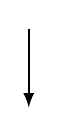
\begin{tikzpicture}
    \draw[-latex,thick](0,0) -- (0,-1); 
  \end{tikzpicture}
\end{center}

\begin{multicols}{2}
  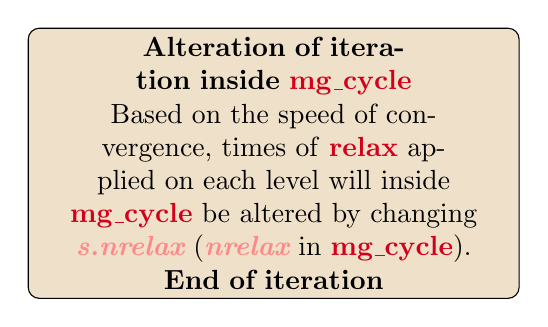
\begin{tikzpicture}
    \node [block](init){
        \textbf{Alteration of iteration inside \func{mg\_cycle}}\\
Based on the speed of convergence, times of \func{relax} applied on each level will inside \func{mg\_cycle} be altered by changing \para{s.nrelax} (\para{nrelax} in \func{mg\_cycle}).\\
\textbf{End of iteration}
      };
  \end{tikzpicture}
  \columnbreak
  \begin{minted}{cpp}
#if 1
    if (s.resa > tolerance) {
      if (resb/s.resa < 1.2 && s.nrelax < 100)
	s.nrelax++;
      else if (resb/s.resa > 10 && s.nrelax > 2)
	s.nrelax--;
    }
#else
    if (s.resa == resb)
      break;
    if (s.resa > resb/1.1 && p.minlevel < grid->maxdepth)
      p.minlevel++;
#endif

    resb = s.resa;
  }
  s.minlevel = minlevel;
  \end{minted}
\end{multicols}

\begin{center}
  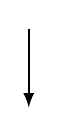
\begin{tikzpicture}
    \draw[-latex,thick](0,0) -- (0,-1); 
  \end{tikzpicture}
\end{center}

\begin{multicols}{2}
  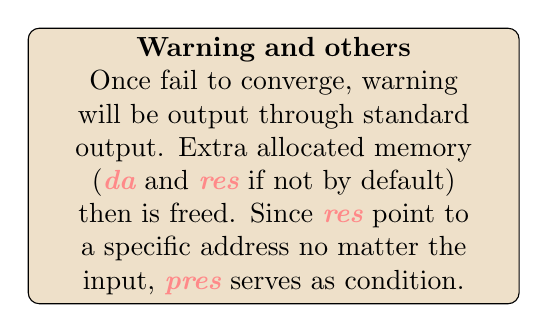
\begin{tikzpicture}
    \node [block](init){
        \textbf{Warning and others}\\
Once fail to converge, warning will be output through standard output. Extra allocated memory (\para{da} and \para{res} if not by default) then is freed. Since \para{res} point to a specific address no matter the input, \para{pres} serves as condition. 
      };
  \end{tikzpicture}
  \columnbreak
  \begin{minted}{cpp}
  if (s.resa > tolerance) {
    scalar v = a[0];
    fprintf (ferr, 
	     "WARNING: convergence for %s not reached after %d iterations\n"
	     "  res: %g sum: %g nrelax: %d tolerance: %g\n", v.name,
	     s.i, s.resa, s.sum, s.nrelax, tolerance), fflush (ferr);
  }
  if (!pres)
    delete (res), free (res);
  delete (da), free (da);

  return s;
}
  \end{minted}
\end{multicols}

\subsection{Poisson-Helmholtz solver}
Now we shall introduce the application for Poisson-Helmholtz equation of multigrid solver.
\subsection{Poisson structure}
\subsubsection{Parameters}
\begin{center}
  \begin{tabular}{|c|c|c|c|c|}
    \hline
    Name & Data type & Status & Option/Default & Representation (before/after)\\[0.5ex]
    \hline\hline
    \para{a} & scalar & unchanged & compulsory & $ \mathbf{a}^{0}$\\
    \hline
    \para{b} & scalar & unchanged & compulsory & $ \mathbf{b} $\\
    \hline
    \para{alpha} & face vector & unchanged & optional/1 & $\alpha$\\
    \hline
    \para{lambda} & scalar & unchanged & optional/0 &  $\lambda$\\
    \hline
    \para{tolerance} & double & unchanged & optional/$10^{-4}$ & $\epsilon$\\
    \hline
    \para{nrelax} & int & unchanged & optional/4 & $n$ \\
    \hline
    \para{minlevel} & int & unchanged & optional/1 & $n$ \\
    \hline
    \para{res} & scalar* & unchanged & optional/NULL & $RES$ \\
    \hline
  \end{tabular}
\end{center}
\subsubsection{Worth Mentioning Details}
Such structure is built for conveying $\alpha$ and $\lambda$ to solve equation \ref{equ:poisson}. \para{res} serves as convergence monitor. \textcolor{red}{anything concerned with embed is under construction}.

\subsubsection{Workflow}
  \begin{minted}{cpp}
struct Poisson {
  scalar a, b;
  (const) face vector alpha;
  (const) scalar lambda;
  double tolerance;
  int nrelax, minlevel;
  scalar * res;
#if EMBED
  double (* embed_flux) (Point, scalar, vector, double *);
#endif
};
  \end{minted}

\subsection{\func{relax}}
\subsubsection{Parameters}
\begin{center}
  \begin{tabular}{|c|c|c|c|c|}
    \hline
    Name & Data type & Status & Option/Default & Representation (before/after)\\[0.5ex]
    \hline\hline
    \rowcolor{output}\para{al} & scalar* & unchanged & compulsory & $ \mathbf{a}^{0}$\\
    \hline
    \para{bl} & scalar* & unchanged & compulsory & $ \mathbf{b} $\\
    \hline
    \para{l} & int & unchanged & compulsory & current level\\
    \hline
    \para{data} & void* & unchanged & compulsory & Poisson data structure \\
    \hline
  \end{tabular}
\end{center}
\subsubsection{Worth Mentioning Details}
Consider the discrete form of equation \ref{equ:poisson} using 5-points Laplacian operator in 2D
\begin{equation}
    \frac{\alpha_{i+\frac{1}{2},j}\frac{a_{i+1,j}-a_{i,j}}{\Delta}-\alpha_{i-\frac{1}{2},j}\frac{a_{i,j}-a_{i-1,j}}{\Delta}}{\Delta}+\frac{\alpha_{i,j+\frac{1}{2}}\frac{a_{i,j+1}-a_{i,j}}{\Delta}-\alpha_{i,j-\frac{1}{2}}\frac{a_{i,j}-a_{i,j-1}}{\Delta}}{\Delta}+\lambda a_{i,j}=b
\end{equation}
and arrange it into forms of equation \ref{equ:indirect} hence the expression of relaxation
\begin{equation}\label{equ:relax}
    a_{i,j}=\frac{\alpha_{i+\frac{1}{2},j}a_{i+1,j}+\alpha_{i-\frac{1}{2},j}a_{i-1,j}+\alpha_{i+\frac{1}{2},j+\frac{1}{2}}a_{i,j+1}+\alpha_{i,j-\frac{1}{2}}a_{i,j-1}-b\Delta^2}{\alpha_{i+\frac{1}{2},j}+\alpha_{i-\frac{1}{2},j}+\alpha_{i,j+\frac{1}{2}}+\alpha_{i,j-\frac{1}{2}}-\lambda\Delta^2}
\end{equation}
By turning on/off macro 'JACOBI', user can choose type of iteration which employed in the solver. Once turning on, solver will implement Jacobi iteration with relaxation factor of $\frac{2}{3}$ i.e. $\mathbf{a}^{n+1}=(\mathbf{a}^{n}+2\mathbf{a}')$. Where $\mathbf{a}'$ is L.H.S. of equation \ref{equ:relax} and will be stored in independent address named \para{c}. If such macro is turned off, \para{c} will be defined as additional pointer pointed to \para{a} and Gauss-Seidel method will be employed. Which indicates equation \ref{equ:indirect} is altered as 
\begin{equation}
\delta x^{k+1}_i = F(\delta x^{k+1}_1,\delta x^{k+1}_2,\cdots,\delta x^{k+1}_{i-1},\delta x^k_{i+1},\cdots,\delta x_n^k, RES^k)  
\end{equation}
and there is no use of relaxation factor.
\subsubsection{Workflow}
\begin{multicols}{2}
  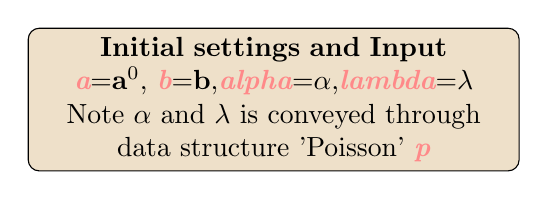
\begin{tikzpicture}
    \node [block](init){
        \textbf{Initial settings and Input}\\
\para{a}=$\mathbf{a}^0$, \para{b}=$\mathbf{b}$,\para{alpha}=$\alpha$,\para{lambda}=$\lambda$\\
Note $\alpha$ and $\lambda$ is conveyed through data structure 'Poisson' \para{p}
      };
  \end{tikzpicture}
  \columnbreak
  \begin{minted}{cpp}
static void relax (scalar * al, scalar * bl, int l, void * data)
{
  scalar a = al[0], b = bl[0];
  struct Poisson * p = (struct Poisson *) data;
  (const) face vector alpha = p->alpha;
  (const) scalar lambda = p->lambda;
  \end{minted}
\end{multicols}

\begin{center}
  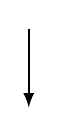
\begin{tikzpicture}
    \draw[-latex,thick](0,0) -- (0,-1); 
  \end{tikzpicture}
\end{center}

\begin{multicols}{2}
  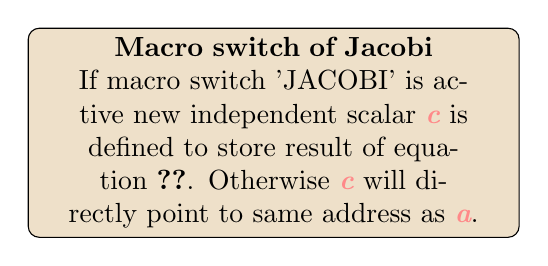
\begin{tikzpicture}
    \node [block](init){
        \textbf{Macro switch of Jacobi}\\
If macro switch 'JACOBI' is active new independent scalar \para{c} is defined to store result of equation \ref{equ:relax}. Otherwise \para{c} will directly point to same address as \para{a}.
      };
  \end{tikzpicture}
  \columnbreak
  \begin{minted}{cpp}
#if JACOBI
  scalar c[];
#else
  scalar c = a;
#endif
  \end{minted}
\end{multicols}

\begin{center}
  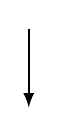
\begin{tikzpicture}
    \draw[-latex,thick](0,0) -- (0,-1); 
  \end{tikzpicture}
\end{center}

\begin{multicols}{2}
  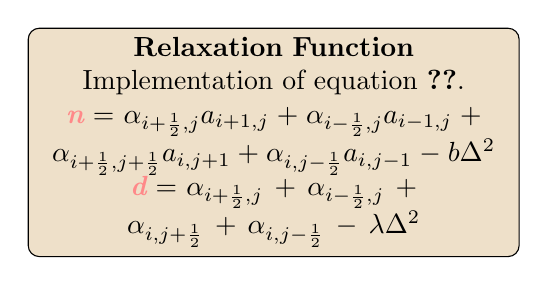
\begin{tikzpicture}
    \node [block](init){
        \textbf{Relaxation Function}\\
Implementation of equation \ref{equ:relax}. \\
\para{n} = $\alpha_{i+\frac{1}{2},j}a_{i+1,j}+\alpha_{i-\frac{1}{2},j}a_{i-1,j}+\alpha_{i+\frac{1}{2},j+\frac{1}{2}}a_{i,j+1}+\alpha_{i,j-\frac{1}{2}}a_{i,j-1}-b\Delta^2$\\
\para{d} = $\alpha_{i+\frac{1}{2},j}+\alpha_{i-\frac{1}{2},j}+\alpha_{i,j+\frac{1}{2}}+\alpha_{i,j-\frac{1}{2}}-\lambda\Delta^2$
      };
  \end{tikzpicture}
  \columnbreak
  \begin{minted}{cpp}
  foreach_level_or_leaf (l) {
    double n = - sq(Delta)*b[], d = - lambda[]*sq(Delta);
    foreach_dimension() {
      n += alpha.x[1]*a[1] + alpha.x[]*a[-1];
      d += alpha.x[1] + alpha.x[];
    }
  \end{minted}
\end{multicols}

\begin{center}
  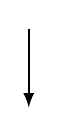
\begin{tikzpicture}
    \draw[-latex,thick](0,0) -- (0,-1); 
  \end{tikzpicture}
\end{center}

\begin{multicols}{2}
  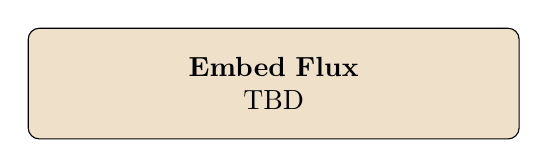
\begin{tikzpicture}
    \node [block](init){
        \textbf{Embed Flux}\\
TBD
      };
  \end{tikzpicture}
  \columnbreak
  \begin{minted}{cpp}
#if EMBED
    if (p->embed_flux) {
      double c, e = p->embed_flux (point, a, alpha, &c);
      n -= c*sq(Delta);
      d += e*sq(Delta);
    }
    if (!d)
      c[] = 0., b[] = 0.;
    else
#endif // EMBED
  \end{minted}
\end{multicols}

\begin{center}
  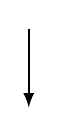
\begin{tikzpicture}
    \draw[-latex,thick](0,0) -- (0,-1); 
  \end{tikzpicture}
\end{center}

\begin{multicols}{2}
  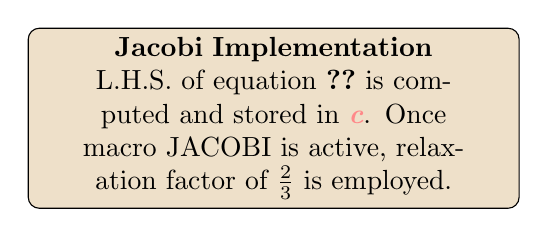
\begin{tikzpicture}
    \node [block](init){
        \textbf{Jacobi Implementation}\\
L.H.S. of equation \ref{equ:relax} is computed and stored in \para{c}. Once macro JACOBI is active, relaxation factor of $\frac{2}{3}$ is employed.
      };
  \end{tikzpicture}
  \columnbreak
  \begin{minted}{cpp}
      c[] = n/d;
  }
#if JACOBI
  foreach_level_or_leaf (l)
    a[] = (a[] + 2.*c[])/3.;
#endif
  
#if TRASH
  scalar a1[];
  foreach_level_or_leaf (l)
    a1[] = a[];
  trash ({a});
  foreach_level_or_leaf (l)
    a[] = a1[];
#endif
}
  \end{minted}
\end{multicols}

\subsection{\func{residual}}
\subsubsection{Parameters}
\begin{center}
  \begin{tabular}{|c|c|c|c|c|}
    \hline
    Name & Data type & Status & Option/Default & Representation (before/after)\\[0.5ex]
    \hline\hline
    \para{al} & scalar* & unchanged & compulsory & $ \mathbf{a}^{k}$\\
    \hline
    \para{bl} & scalar* & unchanged & compulsory & $ \mathbf{b} $\\
    \hline
    \rowcolor{output}\para{resl} & scalar* & unchanged & compulsory & $RES^{k}$\\
    \hline
    \para{l} & int & unchanged & compulsory & current level\\
    \hline
    \para{data} & void* & unchanged & compulsory & Poisson data structure \\
    \hline
  \end{tabular}
\end{center}
\subsubsection{Worth Mentioning Details}
The function aim to solve 
\begin{equation}\label{equ:res}
    RES^k=b_{i,j}-\frac{\alpha_{i+\frac{1}{2},j}\frac{a_{i+1,j}^k-a^k_{i,j}}{\Delta}-\alpha_{i-\frac{1}{2},j}\frac{a^k_{i,j}-a^k_{i-1,j}}{\Delta}}{\Delta}-\frac{\alpha_{i,j+\frac{1}{2}}\frac{a^k_{i,j+1}-a^k_{i,j}}{\Delta}-\alpha_{i,j-\frac{1}{2}}\frac{a^k_{i,j}-a^k_{i,j-1}}{\Delta}}{\Delta}-\lambda a^k_{i,j}
\end{equation}
however careful consideration is needed when it comes to tree grid. Same problem has been fully discussed in section 2.3.2 of 'viscosity.h Documentation' and will not be repeated here.\par
The maximum residual is returned by \func{residual} and serves as criterion in \func{mg\_solve} as described in section \ref{sec:mgsolver}.

\subsubsection{Workflow}
\begin{multicols}{2}
  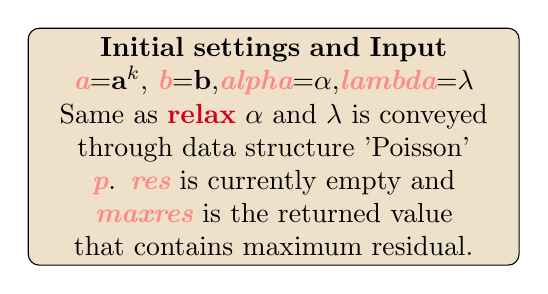
\begin{tikzpicture}
    \node [block](init){
        \textbf{Initial settings and Input}\\
\para{a}=$\mathbf{a}^k$, \para{b}=$\mathbf{b}$,\para{alpha}=$\alpha$,\para{lambda}=$\lambda$\\
Same as \func{relax} $\alpha$ and $\lambda$ is conveyed through data structure 'Poisson' \para{p}. \para{res} is currently empty and \para{maxres} is the returned value that contains maximum residual. 
      };
  \end{tikzpicture}
  \columnbreak
  \begin{minted}{cpp}
static double residual (scalar * al, scalar * bl, scalar * resl, void * data)
{
  scalar a = al[0], b = bl[0], res = resl[0];
  struct Poisson * p = (struct Poisson *) data;
  (const) face vector alpha = p->alpha;
  (const) scalar lambda = p->lambda;
  double maxres = 0.;
  \end{minted}
\end{multicols}

\begin{center}
  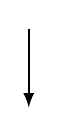
\begin{tikzpicture}
    \draw[-latex,thick](0,0) -- (0,-1); 
  \end{tikzpicture}
\end{center}

\begin{multicols}{2}
  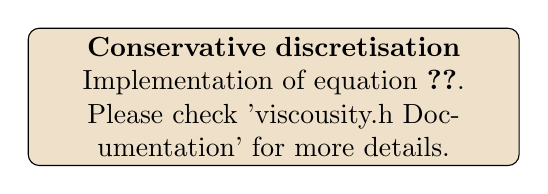
\begin{tikzpicture}
    \node [block](init){
        \textbf{Conservative discretisation}\\
Implementation of equation \ref{equ:res}. Please check 'viscousity.h Documentation' for more details.
      };
  \end{tikzpicture}
  \columnbreak
  \begin{minted}{cpp}
#if TREE
  face vector g[];
  foreach_face()
    g.x[] = alpha.x[]*face_gradient_x (a, 0);
  foreach (reduction(max:maxres), nowarning) {
    res[] = b[] - lambda[]*a[];
    foreach_dimension()
      res[] -= (g.x[1] - g.x[])/Delta;
  \end{minted}
\end{multicols}

\begin{center}
  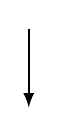
\begin{tikzpicture}
    \draw[-latex,thick](0,0) -- (0,-1); 
  \end{tikzpicture}
\end{center}

\begin{multicols}{2}
  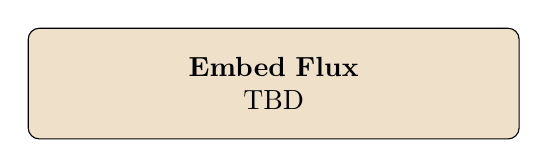
\begin{tikzpicture}
    \node [block](init){
        \textbf{Embed Flux}\\
TBD
      };
  \end{tikzpicture}
  \columnbreak
  \begin{minted}{cpp}
#if EMBED
    if (p->embed_flux) {
      double c, e = p->embed_flux (point, a, alpha, &c);
      res[] += c - e*a[];
    }
#endif // EMBED 
  \end{minted}
\end{multicols}

\begin{center}
  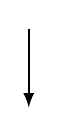
\begin{tikzpicture}
    \draw[-latex,thick](0,0) -- (0,-1); 
  \end{tikzpicture}
\end{center}

\begin{multicols}{2}
  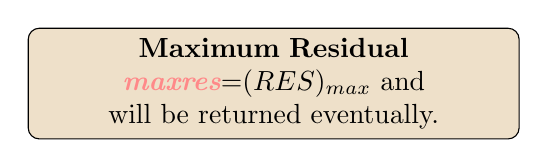
\begin{tikzpicture}
    \node [block](init){
        \textbf{Maximum Residual}\\
\para{maxres}=$(RES)_{max}$ and will be returned eventually.
      };
  \end{tikzpicture}
  \columnbreak
  \begin{minted}{cpp}
    if (fabs (res[]) > maxres)
      maxres = fabs (res[]);
  }
  \end{minted}
\end{multicols}

\begin{center}
  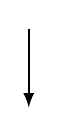
\begin{tikzpicture}
    \draw[-latex,thick](0,0) -- (0,-1); 
  \end{tikzpicture}
\end{center}

\begin{multicols}{2}
  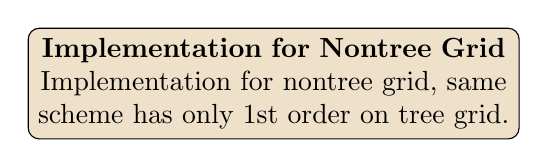
\begin{tikzpicture}
    \node [block](init){
        \textbf{Implementation for Nontree Grid}\\
Implementation for nontree grid, same scheme has only 1st order on tree grid.
      };
  \end{tikzpicture}
  \columnbreak
  \begin{minted}{cpp}
#else
  foreach (reduction(max:maxres), nowarning) {
    res[] = b[] - lambda[]*a[];
    foreach_dimension()
      res[] += (alpha.x[0]*face_gradient_x (a, 0) -
		alpha.x[1]*face_gradient_x (a, 1))/Delta;  
#if EMBED
    if (p->embed_flux) {
      double c, e = p->embed_flux (point, a, alpha, &c);
      res[] += c - e*a[];
    }
#endif
    if (fabs (res[]) > maxres)
      maxres = fabs (res[]);
  }
  \end{minted}
\end{multicols}

\begin{center}
  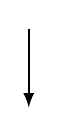
\begin{tikzpicture}
    \draw[-latex,thick](0,0) -- (0,-1); 
  \end{tikzpicture}
\end{center}

\begin{multicols}{2}
  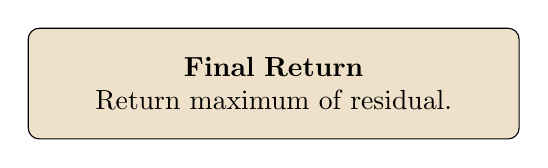
\begin{tikzpicture}
    \node [block](init){
        \textbf{Final Return}\\
Return maximum of residual.
      };
  \end{tikzpicture}
  \columnbreak
  \begin{minted}{cpp}
#endif
  return maxres;
}
  \end{minted}
\end{multicols}
\printbibliography
\end{document}
